\documentclass[12pt,a4paper]{amsart}
\usepackage{amsfonts}
\usepackage{amssymb}
\usepackage{amsbsy}
\usepackage{amsmath}
\usepackage{accents}
\usepackage{array}
\usepackage{mathrsfs}
\usepackage{graphicx}
\usepackage{color}
\usepackage{units}
\usepackage{longtable}
\usepackage{caption}
\usepackage{harvard}
\PassOptionsToPackage{hyphens}{url}\usepackage{hyperref}
\usepackage[titletoc,title]{appendix}
\usepackage{xcolor}
\hypersetup{
    colorlinks,
    linkcolor={red!50!black},
    citecolor={blue!50!black},
    urlcolor={blue!80!black}
}





%-------------------- GET PROPER LAELS AND REFERENCING FOR DESCRIPTION LISTS ----------------------
\makeatletter
\newcommand{\labitem}[2]{%
\def\@itemlabel{\textbf{#1}}
\item
\def\@currentlabel{#1}\label{#2}}
\makeatother


%-------------------- SOME USEFUL DIMENSION SETTING FOR TALES --------------------------------
\setlength{\extrarowheight}{0.2cm}
\setlength{\arraycolsep}{0.08cm}

%-------------------- THEOREM/PROPOSITION COMMANDS -----------------------

\newtheorem{theorem}{Theorem}
\newtheorem{lemma}[theorem]{Lemma}
\newtheorem{proposition}[theorem]{Proposition}
\newtheorem{corollary}[theorem]{Corollary}
\newtheorem{assumption}{Assumptions}

\renewenvironment{proof}[1][Proof]{\begin{trivlist}
\item[\hskip \labelsep {\bfseries #1}]}{\end{trivlist}}
\newenvironment{definition}[1][Definition]{\begin{trivlist}
\item[\hskip \labelsep {\bfseries #1}]}{\end{trivlist}}
\newenvironment{example}[1][Example]{\begin{trivlist}
\item[\hskip \labelsep {\bfseries #1}]}{\end{trivlist}}
\newenvironment{remark}[1][Remark]{\begin{trivlist}
\item[\hskip \labelsep {\bfseries #1}]}{\end{trivlist}}

%----------------- STANDARD COMMANDS -------------------------------------

\renewcommand{\a}{\alpha}
\renewcommand{\b}{\beta}
\renewcommand{\c}{\xi}
\renewcommand{\d}{\delta}
\newcommand{\e}{\epsilon}
\newcommand{\f}{\phi}
\newcommand{\g}{\gamma}
\newcommand{\h}{\eta}
\renewcommand{\i}{\iota}
\renewcommand{\j}{\varphi}
\renewcommand{\k}{\kappa}
\renewcommand{\l}{\lambda}
\newcommand{\m}{\mu}
\newcommand{\n}{\nu}
\newcommand{\p}{\pi}
\renewcommand{\r}{\rho}
\newcommand{\s}{\sigma}
\newcommand{\q}{\theta}
\renewcommand{\t}{\tau}
\renewcommand{\u}{\upsilon}
\newcommand{\w}{\omega}
\newcommand{\x}{\chi}
\newcommand{\y}{\psi}
\newcommand{\z}{\zeta}
\newcommand{\D}{\Delta}
\newcommand{\F}{\Phi}
\newcommand{\G}{\Gamma}
\renewcommand{\L}{\Lambda}
\newcommand{\Q}{\Theta}
\renewcommand{\S}{\Sigma}
\newcommand{\W}{\Omega}
\newcommand{\Y}{\Psi}
\newcommand{\bgtilde}[1]{\tilde{\bg #1}}					%overset tilde bolded little greek letter
\newcommand{\bghat}[1]{\hat{\bg #1}}						%overset hat bolded little greek letter
\newcommand{\btilde}[1]{\tilde{\bm #1}}					%overset tilde on bolded letter
\newcommand{\bhat}[1]{\hat{\bm #1}}						%overset hat on bolded letter
\newcommand{\ds}{\displaystyle}							%force display maths formatting on inline equation
\renewcommand{\bf}{\textbf}								%bold font in text
\newcommand{\bm}{\mathbf}								%bold font in maths
\newcommand{\bg}{\boldsymbol}							%bold font in maths for small greek letters
\newcommand{\tf}{\textrm}								%text font in maths
\newcommand{\Def}[1]{\bf{Definition (#1):}}				%generic "definition" macro
\newcommand{\dd}[1]{\frac{\partial}{\partial #1}}		%Used for taking partial derivatives
\newcommand{\ddt}[1]{\frac{\partial^2}{\partial {#1}^2}}	%Used for taking second partial derivative
\newcommand{\dsqd}[1]{\frac{\partial^2}{\partial #1}}	%Used for taking second partial derivatives
\newcommand{\independent}{\protect\mathpalette{\protect\independenT}{\perp}}	%independence symbol
\def\independenT#1#2{\mathrel{\rlap{$#1#2$}\mkern2mu{#1#2}}}				%independence symbol (cont'd)
\newcommand{\cov}{\textrm{cov}}							%covariance
\newcommand{\Acov}{\textrm{Acov}}						%aymptotic covariance
\renewcommand{\skew}{\textrm{skew}}						%skewness
\newcommand{\kurt}{\textrm{kurt}}						%kurtosis
\newcommand{\plim}{\textrm{plim}}						%probability limit
\newcommand{\as}{\textrm{a.s.}}							%almost surely
\newcommand{\ms}{\textrm{m.s.}}							%mean square
\newcommand{\ConT}{\overset{T \rightarrow \infty}{\xrightarrow{\hspace*{0.75cm}}}} %converges T goes to infinity
\newcommand{\ConN}{\overset{N \rightarrow \infty}{\xrightarrow{\hspace*{0.75cm}}}} %converges N goes to infinity
\newcommand{\ConP}{\overset{\P}{\longrightarrow}}		%converges in probability
\newcommand{\ConAS}{\overset{\as}{\longrightarrow}}		%converges almost surely
\newcommand{\ConMS}{\overset{\ms}{\longrightarrow}}		%converges in mean square
\newcommand{\ConD}{\overset{\tf{d}}{\longrightarrow}}	%converges in distribution
\newcommand{\ConLOne}{\overset{\mathcal{L}_1}{\longrightarrow}}		%converges in L1
\newcommand{\ConLTwo}{\overset{\mathcal{L}_2}{\longrightarrow}}	%converges in L1
\newcommand{\WLLN}[3]{\lim_{#1} \P \left( #2 - #3 > \e \right) < \d, \forall \e, \d > 0}	%Denotes a weak law of large numbers
\newcommand{\SLLN}[3]{\P \left( \lim_{#1} #2 = #3 \right) = 1}	%Denotes a strong law of large numbers
\newcommand{\limN}{\lim_{N \rightarrow \infty}}			%A common limit
\newcommand{\limD}{\lim_{\D \rightarrow 0}}				%A common limit
\newcommand{\limh}{\lim_{h \rightarrow \infty}}			%A common limit
\newcommand{\ADis}{\overset{\tf{a}}{\backsim}}			%asymptotically distributed as
\newcommand{\iidDis}{\overset{iid}{\backsim}}           %iid distributed as
\newcommand{\N}{\mathcal{N}}							%normal distribution "N"
\newcommand{\norm}[1]{\left|\left| #1 \right|\right|}		%norm
\newcommand{\abs}[1]{\left| #1 \right|}				 	%absolute value
\newcommand{\tran}{\mathsf{T}}							%transpose
\newcommand{\tr}{\mathrm{tr}}							%trace
\newcommand{\adj}{\mathrm{adj}}							%adjoint (of a matrix)
\newcommand{\sign}{\mathrm{sign} \:}               		%the sign of a number
\newcommand{\sumtT}{\sum_{t=1}^T}						%sum from t to T
\newcommand{\sumsT}{\sum_{s=1}^T}						%sum from s to T
\newcommand{\sumnN}{\sum_{n=1}^N}						%sum from n to N
\newcommand{\summN}{\sum_{m=1}^N}
\newcommand{\sumkK}{\sum_{k=1}^K}						%sum from k to K
\newcommand{\sumin}{\sum_{i=1}^n}						%sum from i to n
\newcommand{\sumiN}{\sum_{i=1}^N}						%sum from i to N
\newcommand{\sumjN}{\sum_{j=1}^N}						%Sum from j to N
\newcommand{\summM}{\sum_{m=1}^M}						%sum from m to M
\newcommand{\sumjJ}{\sum_{j=1}^J}						%sum from j to J
\newcommand{\prodtT}{\prod_{t=1}^T}						%prod from t to T
\newcommand{\prodnN}{\prod_{n=1}^N}						%prod from n to N
\newcommand{\prodkK}{\prod_{k=1}^K}						%prod from k to K
\newcommand{\prodin}{\prod_{i=1}^n}						%prod from i to n
\newcommand{\intn}{\int_{t_0}^{t_n}}					%integral from t_0 to t_n
\newcommand{\intN}{\int_{t_0}^{t_N}}					%integral from t_0 to t_N
\newcommand{\inti}{\int_{t_0}^{t_i}}					%integral from t_0 to t_i
\newcommand{\intimi}{\int_{t_{i-1}}^{t_i}}				%integral from t_{i-1} to t_i
\renewcommand{\P}{\mathbb{P}}							%blackboard style "P" for probability
\newcommand{\E}{\mathbb{E}}								%blackboard style "E" for expecatation
\newcommand{\V}{\mathbb{V}}								%blackboard style "V" for variance
\newcommand{\R}{\mathbb{R}}								%blackboard style "R" to denote real number line
\newcommand{\CalF}{\mathcal{F}}							%mathcal style "F" to denote filtration
\newcommand{\CalG}{\mathcal{G}}							%mathcal style "G" to denote a grid
\newcommand{\CalH}{\mathcal{H}}							%mathcal style "H" to denote a sub-grid
\newcommand{\CalA}{\mathcal{A}}							%mathcal style "A" to denote some set
\newcommand{\CalB}{\mathcal{B}}							%mathcal style "B" to denote some set
\newcommand{\CalD}{\mathcal{D}}							%mathcal style "D" to denote some set
\newcommand{\CalI}{\mathcal{I}}							%mathcal style "I" to denote a set
\newcommand{\CalL}{\mathcal{L}}							%mathcal style "L" used to denote boundedness
\newcommand{\CalV}{\mathcal{V}}						%mathcal style "V" to denote some set
\newcommand{\CalP}{\mathcal{P}}							%mathcal style "P" to denote some set
\newcommand{\CalN}{\mathcal{N}}							%mathcal style "N" for denoting the normal distribution
\newcommand{\CalT}{\mathcal{T}}							%mathcal style "T" to denote some set
\newcommand{\CalX}{\mathcal{X}}							%mathcal style "X" to denote a set (usually of observations)
\newcommand{\ScrF}{\mathscr{F}}							%mathscr style "F" to denote filtration
\newcommand{\ScrG}{\mathscr{G}}							%mathscr style "G" to denote a grid
\newcommand{\ScrH}{\mathscr{H}}							%mathscr style "H" to denote a sub-grid
\newcommand{\ScrA}{\mathscr{A}}							%mathscr style "A" to denote some set
\newcommand{\ScrB}{\mathscr{B}}							%mathscr style "B" to denote some set
\newcommand{\ScrD}{\mathscr{D}}							%mathscr style "D" to denote some set
\newcommand{\ScrI}{\mathscr{I}}							%mathscr style "I" to denote some set
\newcommand{\ScrL}{\mathscr{L}}							%mathscr style "L" used to denote boundedness
\newcommand{\ScrV}{\mathscr{V}}							%mathscr style "V" to denote some set
\newcommand{\ScrP}{\mathscr{P}}							%mathscr style "P" to denote some set
\newcommand{\ScrN}{\mathscr{N}}							%mathscr style "N" for denoting the normal distribution
\newcommand{\FrakL}{\mathfrak{L}}						%mathfrak style "L" to denote a likelihood function
\newcommand{\Fraks}{\mathfrak{s}}						%mathfrak style "s"
\newcommand{\frakf}{\mathfrak{f}}						%mathfrak style "f"
\newcommand{\frakp}{\mathfrak{p}}                     %mathfrak style "p"
\newcommand{\can}{\citeasnoun}							%Used as a shortcut for the citation command
\newcommand{\blue}[1]{{\color{blue}#1}}					%Used to get blue text
\newcommand{\red}[1]{{\color{red}#1}}					%Used to get red text
\newcommand{\green}[1]{{\color{green}#1}}				%Used to get green text
\newcommand{\ra}{\rightarrow}							%Shorthand for right arrow
\newcommand{\qh}{\hatlatex article abstract{\theta}}							%Used to denote an estimator
\newcommand{\nh}{\hat{\n}}								%Used to denote an estimator
\newcommand{\ellb}{\bar{\ell}}							%Used to denote the scaled log likelihood
\newcommand{\qb}{\bar{q}}								%Used to denote the scaled score
\newcommand{\Qb}{\bar{Q}}								%Used to denote the scaled hessian
\newcommand{\fbrac}[1]{\f \left( #1 \right)}			%Used for the standard normal
\newcommand{\Fbrac}[1]{\F \left( #1 \right)}			%Used for the cumulative normal
\newcommand{\ebrac}[1]{\exp \left( #1 \right)}			%Used for the exponential function
\newcommand{\half}{\frac{1}{2}}							%Shorthand for a half
\newcommand{\mhalf}{-\frac{1}{2}}						%Shorthand for minus a half

%----------------------- CUSTOM DOCUMENT COMMANDS ------------------------------------------------




%---------------------------------------------------------------------------


\begin{document}
\title{Bootstrapping Daily Returns}

\author[C. Bowers]{Colin T. Bowers$^\dag$}
\thanks{$^\dag$Department of Economics, Macquarie University, North Ryde NSW 2109, Australia.  \textit{Email:} colintbowers@gmail.com}

\keywords{Robust, Statistics, Non-Gaussian}

\date{5th August, 2016}

\maketitle

\begin{abstract}
This paper is designed to accompany a set of presentation slides that provide a selective introduction to Robust Statistics with a particular focus on financial applications. The topic of robust statistics is introduced, and then methods for measuring fat-tails in the data generating process are discussed. Next, a robust estimator of location, the trimmed mean, is defined, and then some simulations demonstrate its suitability for use with daily financial returns. Finally, robust estimation of a linear model is defined, and then investigated by a series of simulations designed to mimic daily financial returns.
\end{abstract}

\section{Basic Example of Robust Statistics}\label{secBasicExample}

The field of Robust Statistics is concerned with statistical methods for use with non-Gaussian data. In particular, Robust Statistics are especially useful when the data generating process is leptokurtotic (i.e. fat-tails). When data exhibits fat-tails, non-robust (i.e. classical) estimators are typically very sensitive to a handful of outlier observations in the tails of Data Generating Process (DGP). The core idea of Robust Statistics is to ignore, or downplay, the effects of these outlier observations. This usually results in more stable estimates that are a closer reflection of the parameters of the DGP.

For example, Figure~\ref{figtDistDataCutoff} contains $20$ observations generated from a Students-t distribution with $2$ degrees of freedom (a well-known, symmetric, fat-tailed distribution), where the horizontal bars partition $2$ observations in each tail. The true mean of the DGP is $0$, while the sample mean is $1.38$. However, the value of this sample mean is heavily influenced by the tail observations that lie outside the horizontal bars. One robust statistic, known as the \emph{trimmed mean}, suggests removing the tail observations from the sample mean calculation. In this example, if we ignore the observations outside the horizontal bars, then the trimmed mean is $0.68$, which is significantly closer to the true mean of the DGP.

\begin{figure}[htbp]
\centering
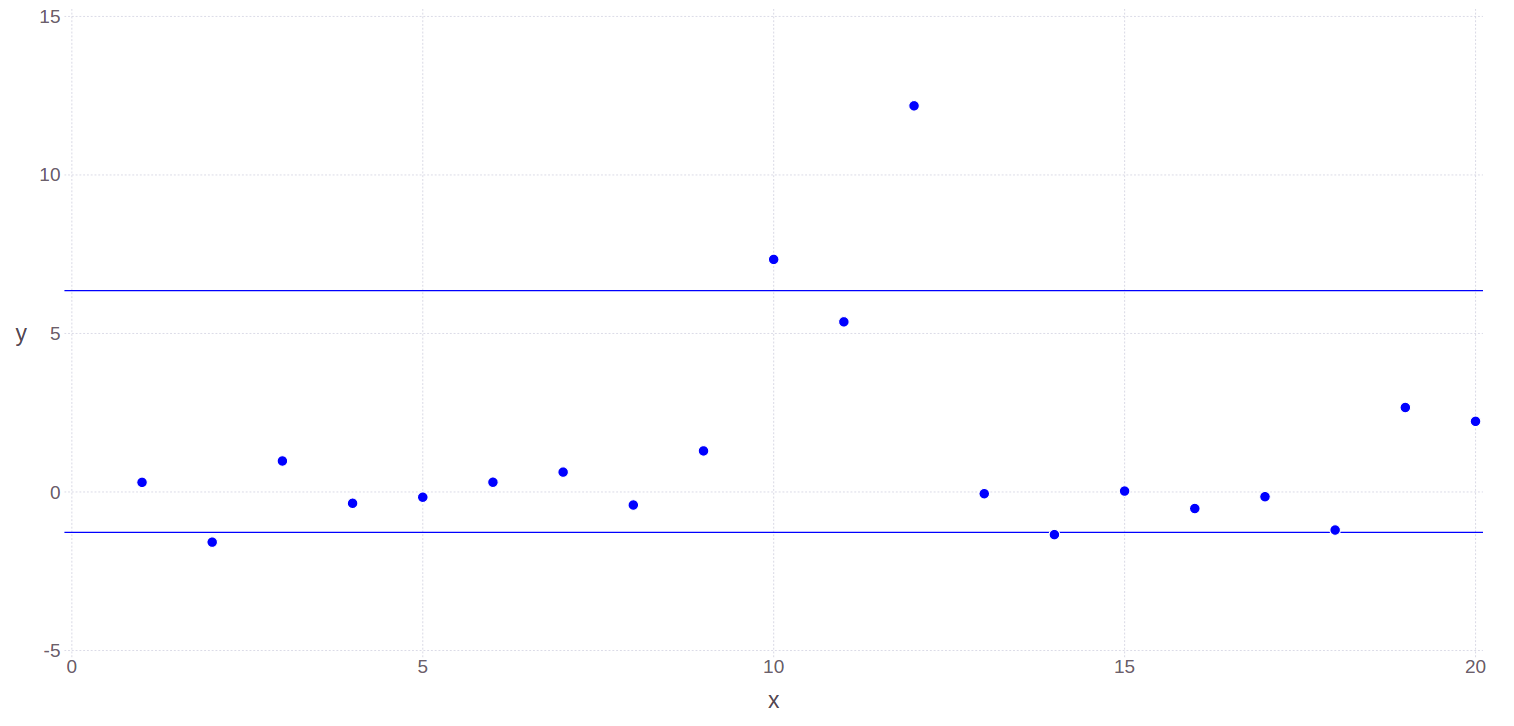
\includegraphics[height=5.35cm]{tDistDataCutoff.png}
\caption{\footnotesize{Data from Student-t distribution with 2 degrees of freedom}}
\label{figtDistDataCutoff}
\end{figure}


The example in the previous paragraph is, of course, cherry-picked for the purposes of illustration. Figure~\ref{figtDistDataEstDensity} provides a more complete picture of the behaviour of different location estimators for Students-t distributed data. Figure~\ref{figtDistDataEstDensity} contains simulated sampling distributions for four different location estimators; the sample mean, the $10$\% trimmed mean, the $50$\% trimmed mean, and the sample median.\footnote{The number of simulation iterations is $5000$, and the number of observations per iteration is 50.} Although all four sampling distributions are centred on the true mean of zero, the sample mean estimates are more likely to be further from zero than estimates from the other three (robust) estimators.

\begin{figure}[htbp]
\centering
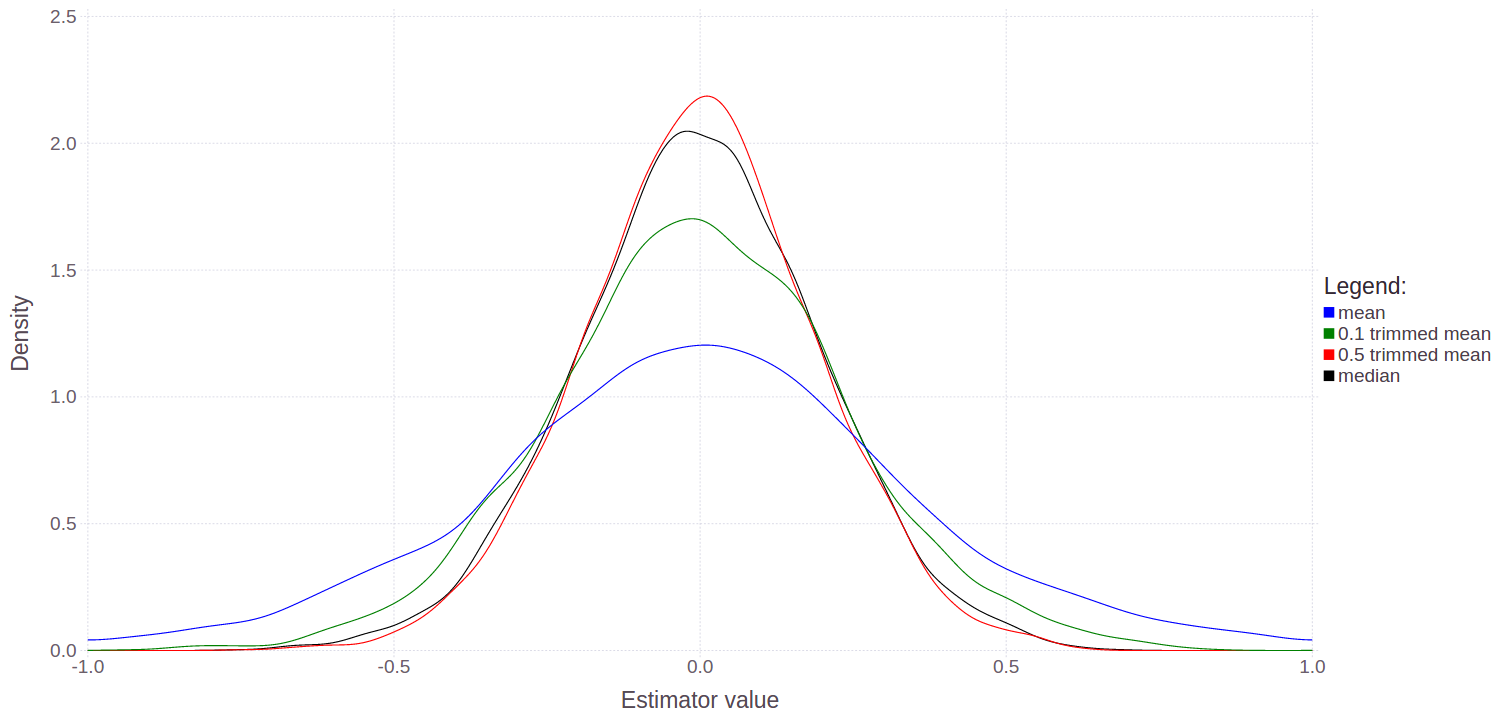
\includegraphics[height=5.35cm]{tDistDataEstDensity.png}
\caption{\footnotesize{Sampling distribution of 4 location estimators}}
\label{figtDistDataEstDensity}
\end{figure}



One other important concept can be gleaned from Figure~\ref{figtDistDataEstDensity}. Note that of the three robust estimators, the $50$\% trimmed mean is, on average, the most accurate. It turns out that there is an optimal\footnote{There are various metrics for optimality, but this is an unnecessary complication at this point.} degree of trimming which depends on the fatness of the tails of the DGP. For the case of Students-t with 2 degrees of freedom, the $10$\% trimmed mean does not trim enough observations, and the median\footnote{The median, by definition, trims all observations except for 1 or 2, depending on whether the total number of observations is odd or even.} trims too many.


\section{Tail Fatness and Kurtosis}\label{secTailFatness}

The example in the previous section demonstrates that Robust Statistics are most useful when the DGP exhibits fat tails. The obvious question is: how do we know if the tails of the DGP are fat? The standard measure of tail fatness is \emph{kurtosis}, i.e. the (scaled) fourth centred moment. The Normal distribution has a kurtosis of $3$, and fat-tailed, or leptokurtotic, distributions have a kurtosis greater than $3$.

Despite its popularity, in my opinion, the kurtosis is not a sensible measure of tail fatness. This is because for distributions with unbounded support (such as the Normal) fatter tails result in undefined higher moments.\footnote{That is, the integrals that define those moments evaluate to $\infty$.} For example, for a Students-t distribution with degrees of freedom $v$, all moments greater than $v$ are undefined. This means that for the Students-t distribution with $2$ degrees of freedom, the variance exists, but the skewness and kurtosis are both undefined.

In summary, if one suspects the data is generated by a fat-tailed DGP, it seems odd to choose a measure of tail fatness whose population parameter is more likely to be undefined in the presence of fat tails.

Fortunately, several robust measures of tail fatness have been proposed. In this paper, I use the measure proposed in \can{Hogg_(1974)}, Section 4. Let $Q(p)$ denote the quantile associated with probability $p$ of some cumulative distribution function $F$ with infinite support. Let:
\begin{equation}
I(a, b) = \int_{Q(a)}^{Q(b)} x dF(x) .
\end{equation}
Then Hogg's robust measure of tail fatness can be defined:
\begin{equation}
\k_{Hogg} = \frac{I(0.95, \infty) - I(-\infty, 0.05)}{I(0.5, \infty) - I(-\infty, 0.5)}
\end{equation}
In words, the numerator is the ``average'' value in the \emph{far right} of the distribution minus the ``average'' value in the \emph{far left}, while the denominator is the ``average'' value in the right minus the ``average'' value in the left. Roughly speaking, the numerator of this measure gets larger as the tails get fatter, while the denominator gets larger as variance increases, and so can be thought of as a scaling factor for controlling for changes in variance.

It is interesting to compare the properties of the robust estimator of tail fatness with the standard sample kurtosis given a Student-t distribution with $2$ degrees of freedom DGP. Figure~\ref{tDistSampleKurtosis} provides simulated average values for these two estimators for various sample sizes. As can be seen, the sample kurtosis diverges with the sample size (a common phenomenon when the population parameter is undefined). In contrast, the robust estimator of fat tails is stable with respect to the sample size, which is a much more desirable property in an estimator.

\begin{figure}[htbp]
\centering
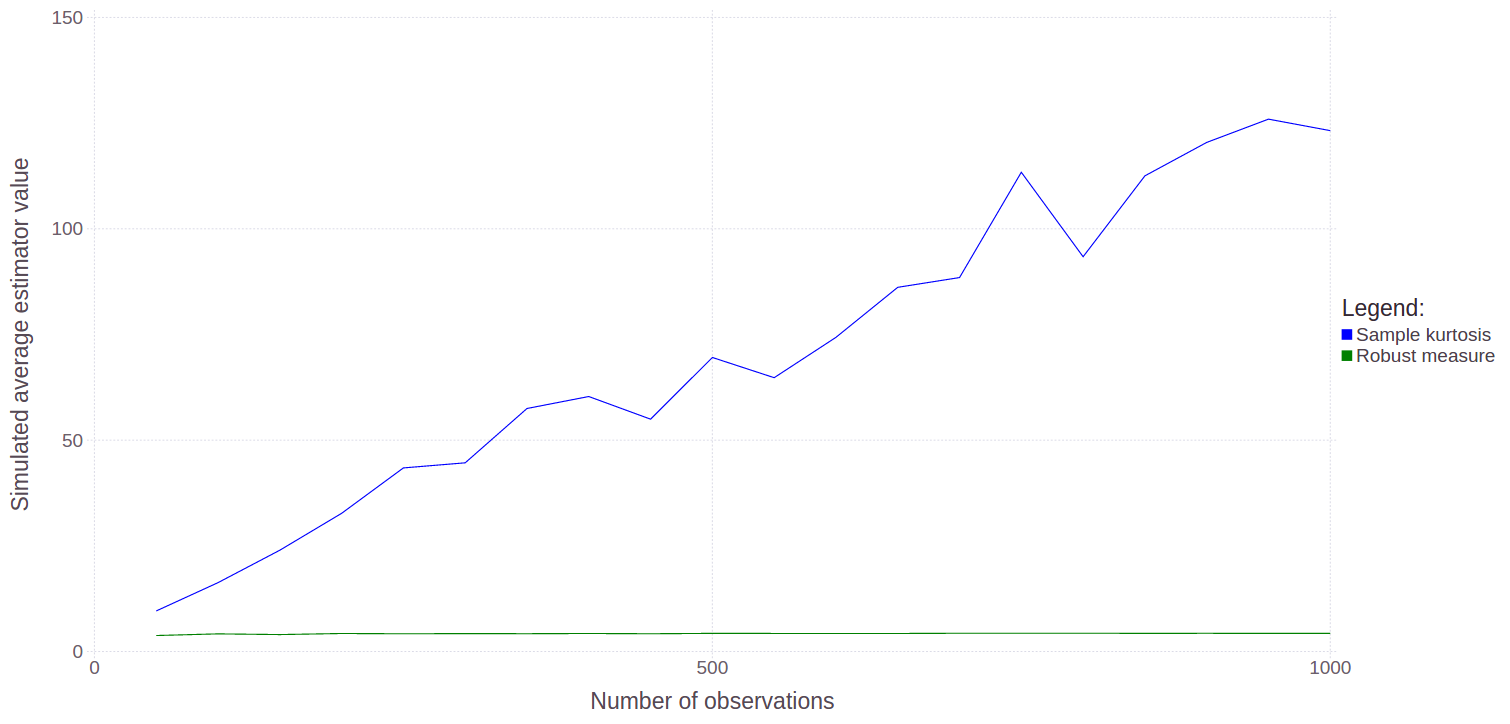
\includegraphics[height=5.35cm]{tDistSampleKurtosis.png}
\caption{\footnotesize{Sample kurtosis as a function of sample size when population kurtosis is undefined}}
\label{figtDistSampleKurtosis}
\end{figure}



\section{Establishing Tail Fatness of Financial Returns}\label{secFinReturnTailFatness}

In this section we examine the tail fatness of daily financial returns. Using daily\footnote{Close to close.} data from January 2005 to December 2015, I calculate Hogg's robust measure of tail fatness for several of the most popular stocks listed on the ASX.\footnote{AMP, ANZ, BHP, CBA, CCL, CWN, JBH, LLC, MQG, NAB, RIO, SUN, TLS, TOL, WBC, WES, WOW.} The estimates are depicted in Figure~\ref{figRobustKurtStocks}, along with two reference lines; one is the population value of Hogg's estimator for the Normal distribution, and the other is for the Student-t distribution with $2$ degrees of freedom. As can be seen, according to Hogg's measure, all the stocks in the sample exhibit fat tails relative to the Normal distribution. This is typical of financial return data.

\begin{figure}[htbp]
\centering
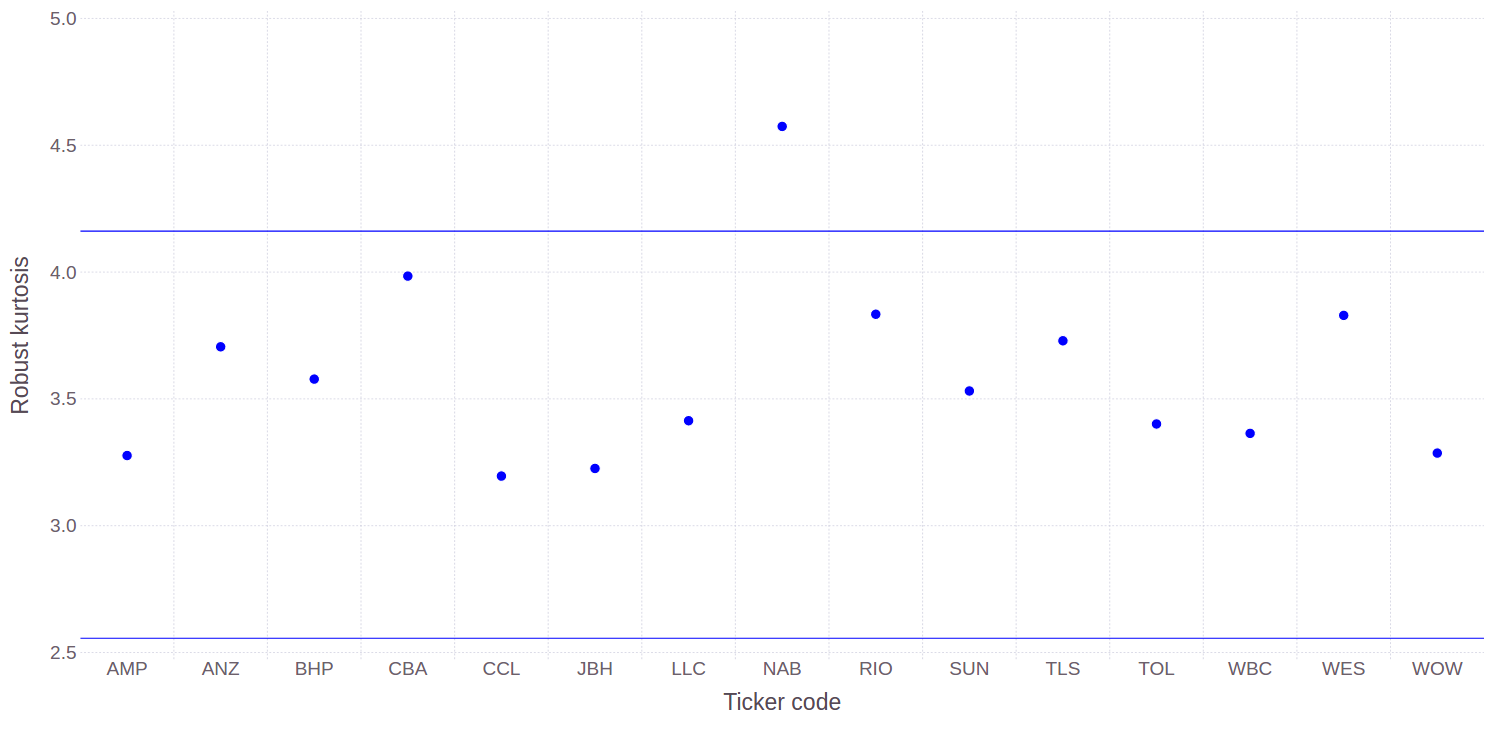
\includegraphics[height=5.35cm]{RobustKurtStocks.png}
\caption{\footnotesize{Robust kurtosis for daily returns of 15 stocks listed on the ASX. The bottom and top reference lines are the population robust kurtosis for the Normal and the Student-t (2 degrees of freedom) distributions respectively.}}
\label{figRobustKurtStocks}
\end{figure}

It is worth briefly diverging here into a quick discussion of how statisticians typically model fat tails in financial returns. One of the most popular approaches is to model returns as Normal, but with a conditional or stochastic volatility, i.e. $r_t | \s_t^2 \backsim \N(\m, \s_t^2)$. This framework will generate an unconditionally fat-tailed sequence. The intuition is fairly simple: a small number of returns generated when $\s_t^2$ is large will, on average, be much further into the tails of the unconditional distribution than when $\s_t^2$ is small. To see this in real world data, one needs to only to plot returns from 2006 to 2009, and note how the returns during the market crash of late 2008 and recovery of early 2009 dominate the sample.

Assuming this modelling framework, it follows that the sequence $r_t / \s_t$ should have constant volatility, and thus not exhibit fat-tails relative to the Normal. Unfortunately, we cannot model $r_t / \s_t$ explicitly, since $\s_t$ is unobservable. However, we can substitute in an estimate for $\s_t$. Figure~\ref{figRobustKurtStocksStd} duplicates Figure~\ref{figRobustKurtStocks} except that now I have replaced daily returns as the input with daily returns standardised by a rolling window historical volatility estimate (with a window length of $100$). As can be seen, this technique is able to remove some, but not all, of the tail fatness in the return DGP. It is possible that there is a secondary source of tail-fatness in the DGP, but it is also possible that the remaining tail fatness is due to inaccuracies in our proxy for the true volatility process.

\begin{figure}[htbp]
\centering
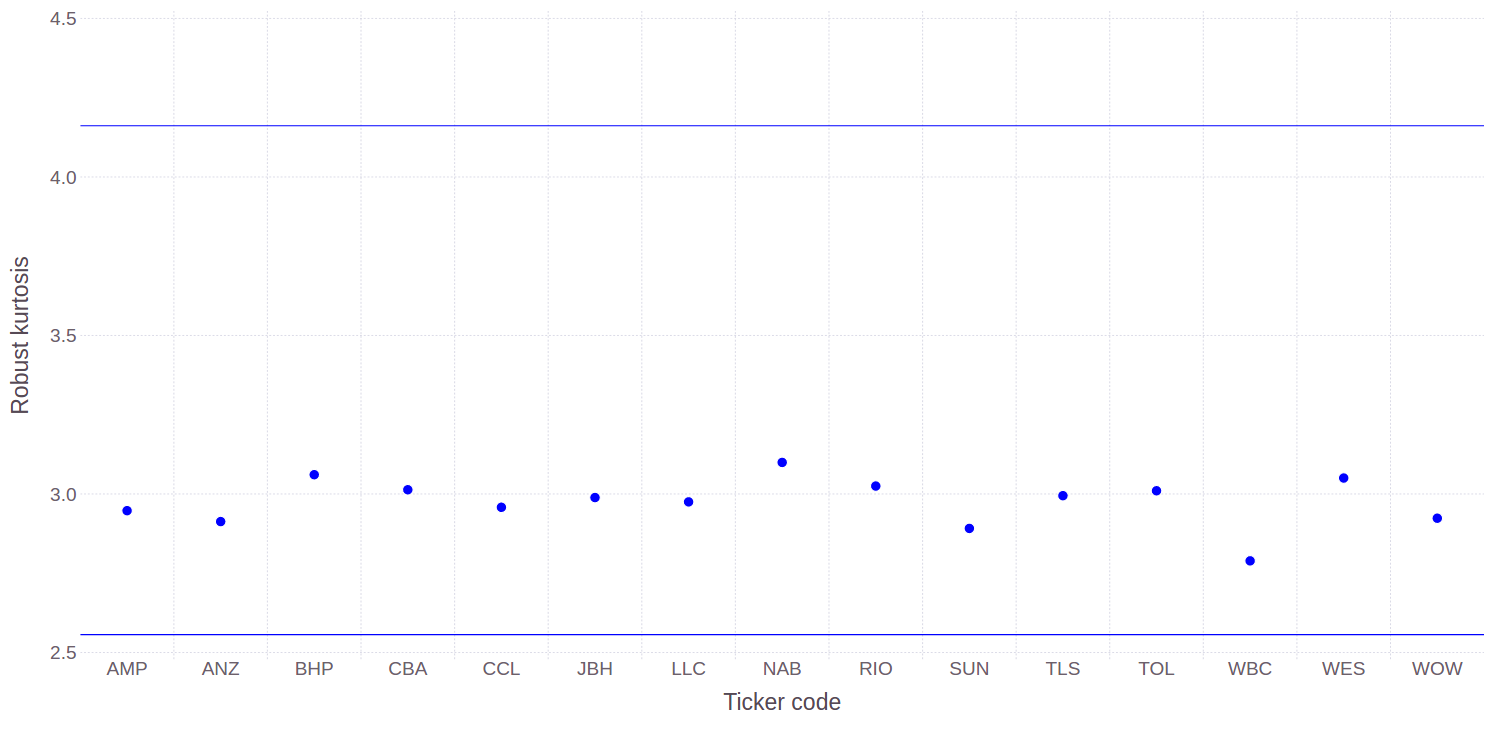
\includegraphics[height=5.35cm]{RobustKurtStocksStd.png}
\caption{\footnotesize{Robust kurtosis standardised daily returns of 15 stocks listed on the ASX. The bottom and top reference lines are the population robust kurtosis for the Normal and the Student-t (2 degrees of freedom) distributions respectively.}}
\label{figRobustKurtStocksStd}
\end{figure}



\section{Robust Estimation of Financial Returns}\label{secFinReturnTailFatness}

Having established the presence of fat tails in financial returns, it is of interest to establish whether practitioners should consider replacing standard statistical estimates with robust statistical estimates. Arguably the most famous estimate in statistics is the sample mean:
\begin{equation}
m_{normal} = \frac{1}{T} \sum_{t=1}^T r_t ,
\end{equation}
which is an estimate of the expected value of a distribution, which is equivalent to the centre of a symmetric distribution. A robust analogue to the sample mean is the trimmed mean. Let $r_{[1]}, ..., r_{[T]}$ denote the sorted version of the sequence $r_1, ..., r_T$ (sometimes called the \emph{order statistics}). Then for some trimming proportion $\a \in [0, 1]$, the trimmed mean is:
\begin{equation}
m_{robust} = \frac{1}{(1 - \a) T} \sum_{t=\frac{\a}{2} T}^{(1 - \frac{\a}{2}) T} r_{[t]} ,
\end{equation}
where for notational convenience I will assume $\a / 2$ is an integer.

In words, the trimmed mean symmetrically removes the largest and smallest $\a / 2$ fraction of observations from the dataset, and then computes a sample mean on the remaining data. Note that for $\a = 0$, the trimmed mean is equivalent to the sample mean, and for $\a = 1$, the trimmed mean is equivalent to the median.

If the underlying DGP is symmetric, then the trimmed mean and sample mean are estimators for the same population statistic. However, if the DGP is fat-tailed, then the trimmed mean is more accurate (on average) than the sample mean as it disregards those observations in the tails of the DGP that add more noise than information. Given the importance of the expected value of financial returns, it is of interest to ask whether the trimmed mean is more accurate when used on financial data than the sample mean. Answering this question is complicated by the fact that the population mean is unobservable. Ideally, what is required is a DGP with roughly the same properties as the DGP for financial returns, but where the population mean is known. Fortunately, we can conjure up such a dataset using a block bootstrap procedure. Full details of the procedure are not provided here, but a classic paper on the subject is \can{Politis_Romano_(1994)}. Intuitively, we take a sequence of financial returns and centre them, so that their sample mean is $0$. We then treat this sequence of returns as if it is the entire population, and resample with replacement from it using a strategy that ensures any weak dependence structure and heteroskedasticity in the data is preserved. By construction, the resampled sequences will have population mean of zero, although their sample means can (and will) differ from zero due to sampling with replacement.

I resample $M$ sequences, each of length $T$, and the nature of the resampling scheme ensures that each sequence is independent from the other sequences. I then calculate both the sample mean and the trimmed mean on each sequence, and from the resulting $M$ estimates can construct a kernel density of the sampling distribution of the estimator. Under certain modelling assumptions, this kernel density will converge on the true asymptotic sampling distribution for the estimator as $\{M, T\} \ra \infty$. I performed this procedure on the sequence of NAB returns, and the sequence of CCL returns. I chose these two assets since in Figure~\ref{figRobustKurtStocks} they have the largest and smallest robust kurtosis (respectively).

As can be seen in Figure~\ref{figNABTrimMeanFullPeriod}, the trimmed mean significantly outperforms the sample mean for NAB data. Perhaps more surprisingly, as Figure~\ref{figCCLTrimMeanFullPeriod} demonstrates, the trimmed mean performance is reasonably good relative to the sample mean even for CCL data. This result is surprising, since CCL has relatively stable volatility over the sample period and so its tails are only mildly fat.

\begin{figure}[htbp]
\centering
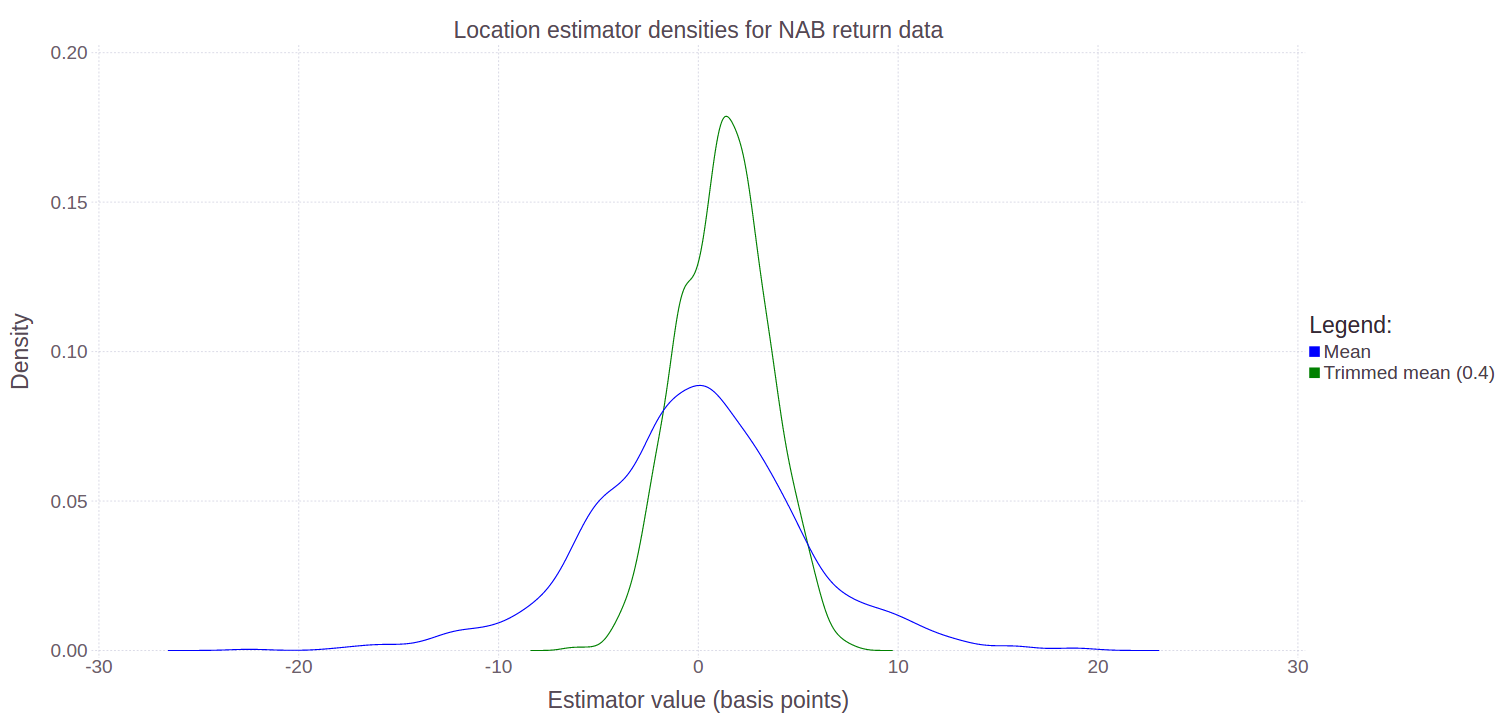
\includegraphics[height=5.35cm]{NABTrimMeanFullPeriod.png}
\caption{\footnotesize{Bootstrapped sampling distributions of the sample mean and trimmed mean when applied to NAB daily return data.}}
\label{figNABTrimMeanFullPeriod}
\end{figure}

\begin{figure}[htbp]
\centering
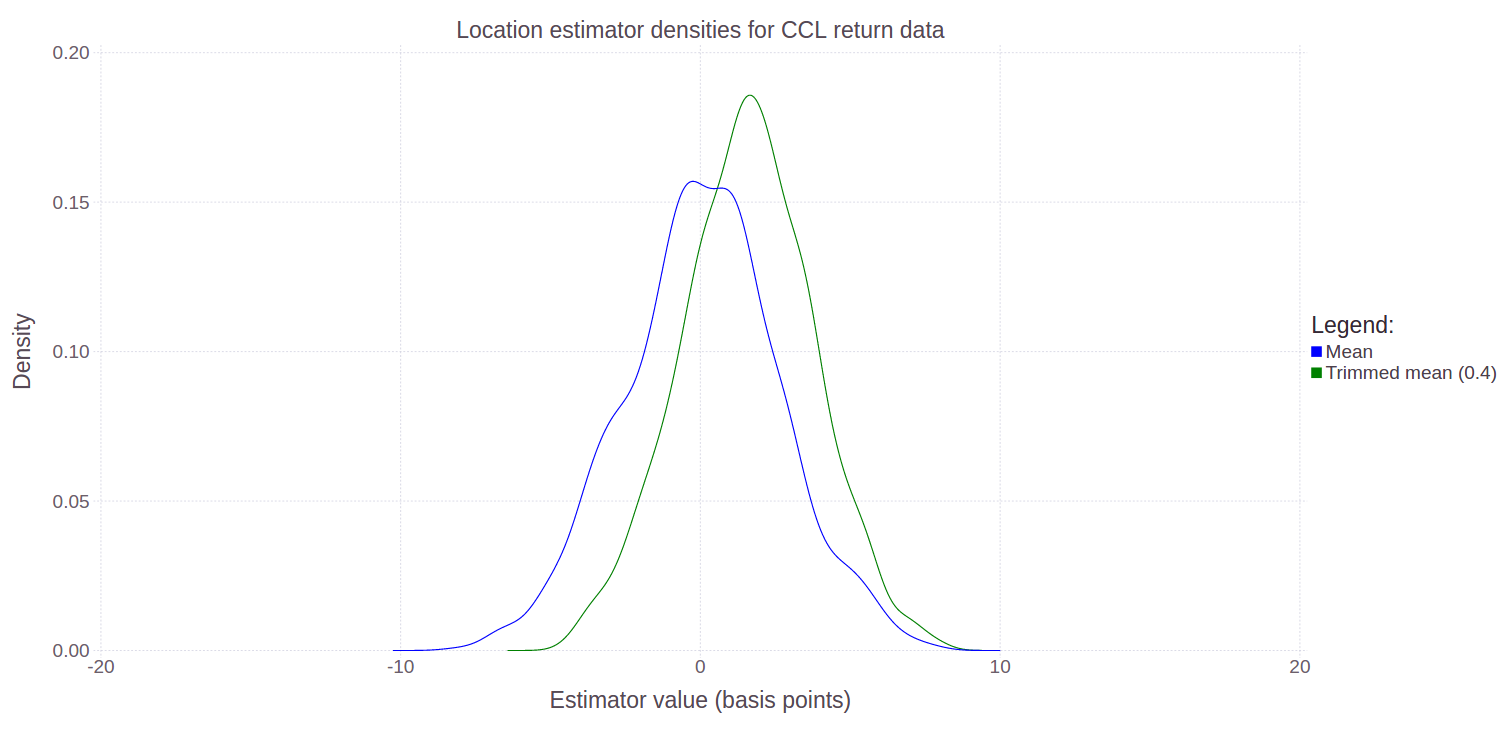
\includegraphics[height=5.35cm]{CCLTrimMeanFullPeriod.png}
\caption{\footnotesize{Bootstrapped sampling distributions of the sample mean and trimmed mean when applied to CCL daily return data.}}
\label{figCCLTrimMeanFullPeriod}
\end{figure}



Note that the sample period in question here is from 2005 to 2015. Of course, this period includes some major financial events, and correspondingly large shifts in volatility. If one chose a shorter horizon, say, $100$ days, perhaps the sample mean would have comparatively better performance, since it is feasible that volatility might be relatively stable over such a short horizon. To investigate this possibility, I isolated the $100$ sequential days in NAB returns that correspond to the largest value of the robust kurtosis, and compare it to the $100$ sequential days that correspond to the smallest robust kurtosis. I perform the same bootstrapping exercise on each of these datasets, and the results are in Figure~\ref{figNABTrimMeanShortFat} and Figure~\ref{figNABTrimMeanShortThin}. As expected, the trimmed mean massively outperforms over the interval with the fattest tails. Indeed, for this interval, the sampling distribution of the sample mean is trimodal! Surprisingly, the sample mean has only slightly better performance for the interval with the thinnest tails.

\begin{figure}[htbp]
\centering
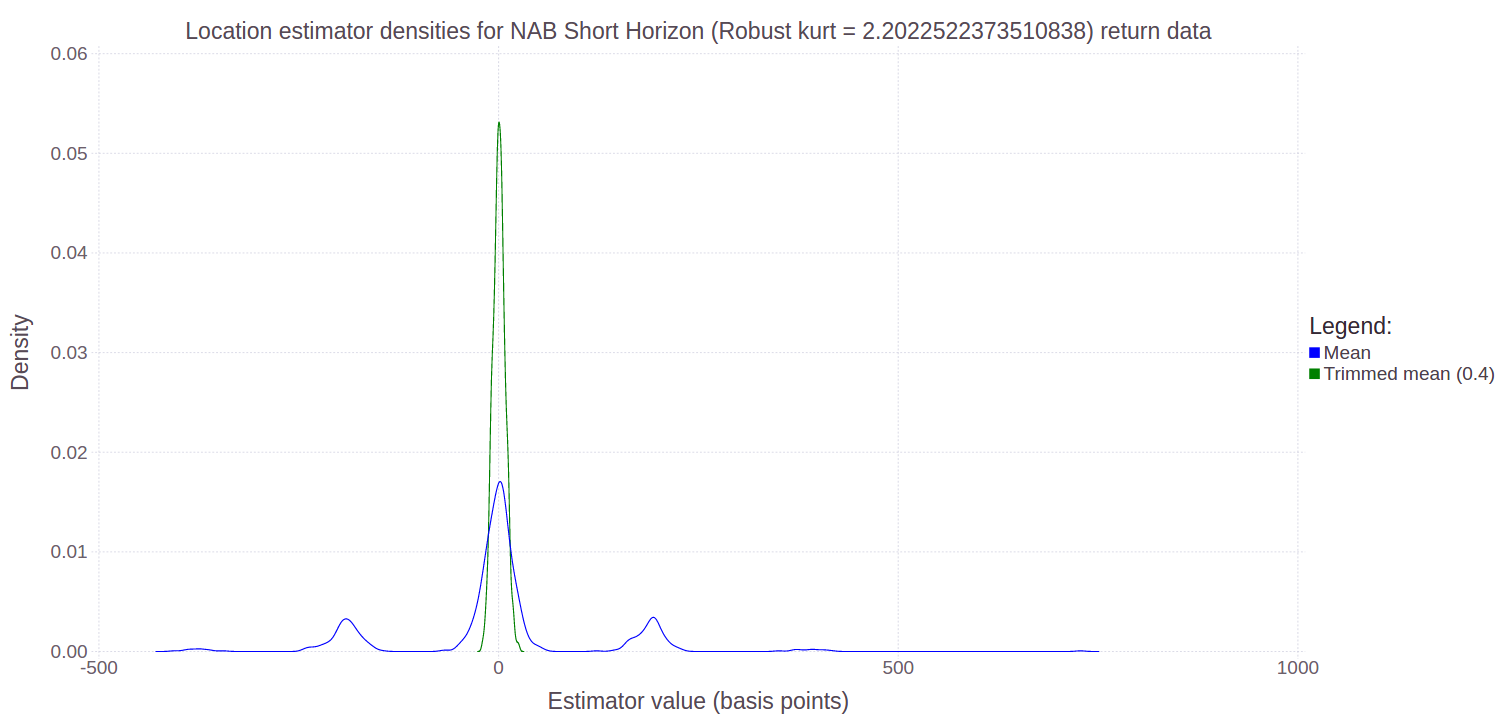
\includegraphics[height=5.35cm]{NABTrimMeanShortFat.png}
\caption{\footnotesize{Bootstrapped sampling distributions of the sample mean and trimmed mean when applied to a short horizon of NAB daily return data with fat tails.}}
\label{figNABTrimMeanShortFat}
\end{figure}

\begin{figure}[htbp]
\centering
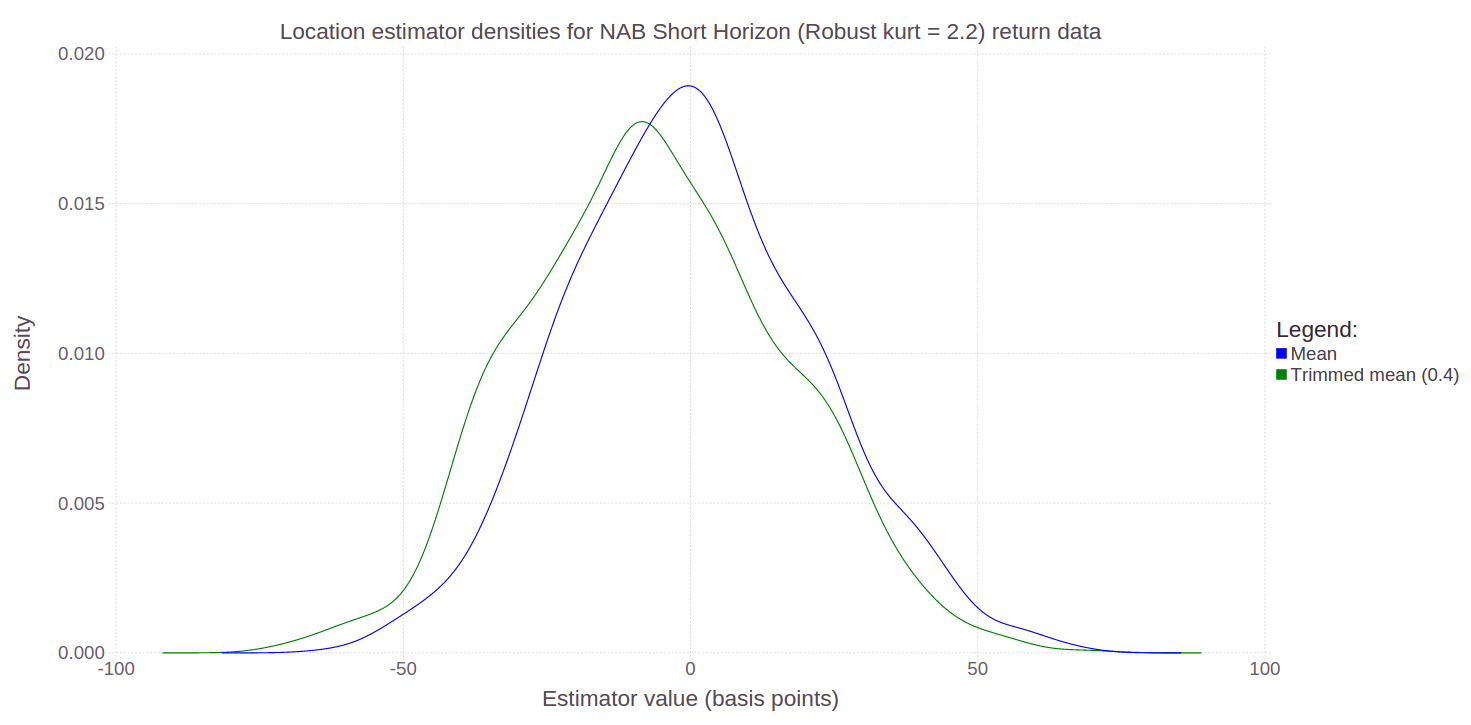
\includegraphics[height=5.35cm]{NABTrimMeanShortThin.png}
\caption{\footnotesize{Bootstrapped sampling distributions of the sample mean and trimmed mean when applied to a short horizon of NAB daily return data with thin tails.}}
\label{figNABTrimMeanShortThin}
\end{figure}




Taken together, the above analysis suggests that a researcher should always at least consider a robust estimate when estimating the first moment of financial returns using historical price data for that asset.


\newpage

\section{Robust Estimation of a Linear Model for Financial Returns}\label{secFinReturnLinearModel}

In this section I examine whether robust estimation methods might be useful for a researcher building a linear model for financial returns. Specifically, I assume the following univariate structure:
\begin{equation}\label{retModel}
r_t = \a + \b s_t + e_t ,
\end{equation}
where $r_t$ is a daily return, $s_t$ is a predictive signal, $e_t$ denotes the residual, and $\{\a, \b\}$ are the parameters of the model.

Given a vector of observable returns $\bm{r}$, and a vector of observable signals $\bm{s}$, the parameters in \eqref{retModel} can be estimated by solving the following optimisation problem:
\begin{equation}
\min_{\a, \b} L(\bm{e}) ,
\end{equation}
where $\bm{e} = \bm{r} - \a - \b \bm{s}$, and $L$ denotes a function for measuring loss. The most popular choice for the loss function is $L(\bm{e}) = \norm{\bm{e}}_2$, i.e. the Euclidean norm, which corresponds to the Ordinary Least Squares (OLS) estimator. It is well understood that if $e_t \backsim \N(0, \s^2)$, then given a few other regularity conditions, OLS yields the best, linear, unbiased estimator.

However, consider the case where $e_t \backsim \N(0, \s_t^2)$, that is, the residuals exhibit a pattern of heteroskedasticity. In this case, the Euclidean norm loss function can place too much emphasis on a small number of observations that correspond to a period of high volatility. It is sometimes better to choose a loss function that places less emphasis on observations that are large in magnitude, such as $L(\bm{e}) = \norm{\bm{e}}_1$, which corresponds to the Least Absolute Deviations (LAD) estimator.\footnote{$\norm{\cdot}_1$ is sometimes called the taxicab norm.}

It is important to note that, unlike Section~\ref{secFinReturnTailFatness}, here it is the statistical properties of the residual, $e_t$, that are important, rather than the statistical properties of the return, $r_t$. However, when predicting financial returns, the $R^2$ associated with a model such as \eqref{retModel} is typically very small, typically much less than $0.05$, and so it is likely that $r_t$ and $e_t$ will have similar statistical properties, such as heteroskedasticity. Thus robust estimators such as the LAD estimator may be of interest.

To investigate the effect of LAD versus OLS, I need to simulate \eqref{retModel} in such a way that $r_t$ exhibits similar statistical properties to real-world financial data. I do this as follows. First, I construct a sequence of variances $\hat{\s}_t^2$, using a rolling historical variance estimator on NAB daily returns. I then simulate the residual term from \eqref{retModel} using the assumption $e_t \backsim \N(0, \hat{\s}_t^2)$. I simulate the signal using $s_t \backsim \N(0, 1)$, set $\a = 0$, and choose $\b$ such that the sample $R^2$ given \eqref{retModel} is $0.05$. Using these inputs and \eqref{retModel}, I then simulate $r_t$. Note that the rolling historical variance estimator, $\hat{\s}_t^2$ can be thought of as a smoothing function on squared NAB returns where a longer window length implies more smoothing, and thus more mild dynamics for $\hat{\s}_t^2$. I deliberately use a window length of $17$ days, as this corresponds to simulated returns $r_t$ that have a robust kurtosis roughly the same as that for a Student-t distribution with $2$ degrees of freedom (the upper line in Figure~\ref{figRobustKurtStocks}).

I simulate $M$ datasets, and for each dataset, I estimate \eqref{retModel} using both the OLS and LAD methodologies. I then construct the kernel density estimates of the sampling distributions of parameter estimates from \eqref{retModel}. As can be seen in Figure~\ref{figConstantDensity} and Figure~\ref{figCoefDensity}, the LAD estimator is significantly more accurate than the OLS estimator for both the constant term and the slope coefficient in \eqref{retModel}. It immediately follows that predictions made using the LAD estimators will, in this framework, be more accurate than their OLS counterparts, on average.

\begin{figure}[htbp]
\centering
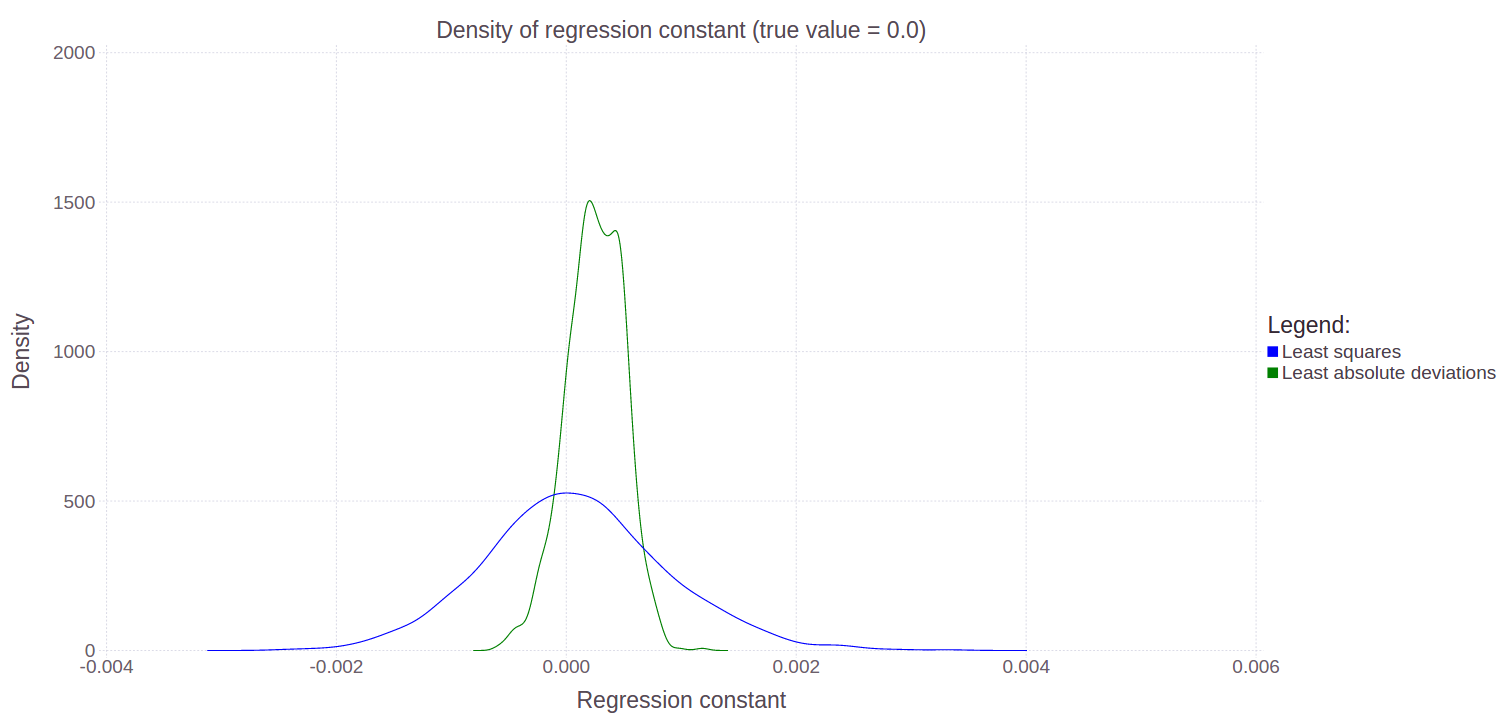
\includegraphics[height=5.35cm]{ConstantDensity.png}
\caption{\footnotesize{Regression constant sampling distribution.}}
\label{figConstantDensity}
\end{figure}



\begin{figure}[htbp]
\centering
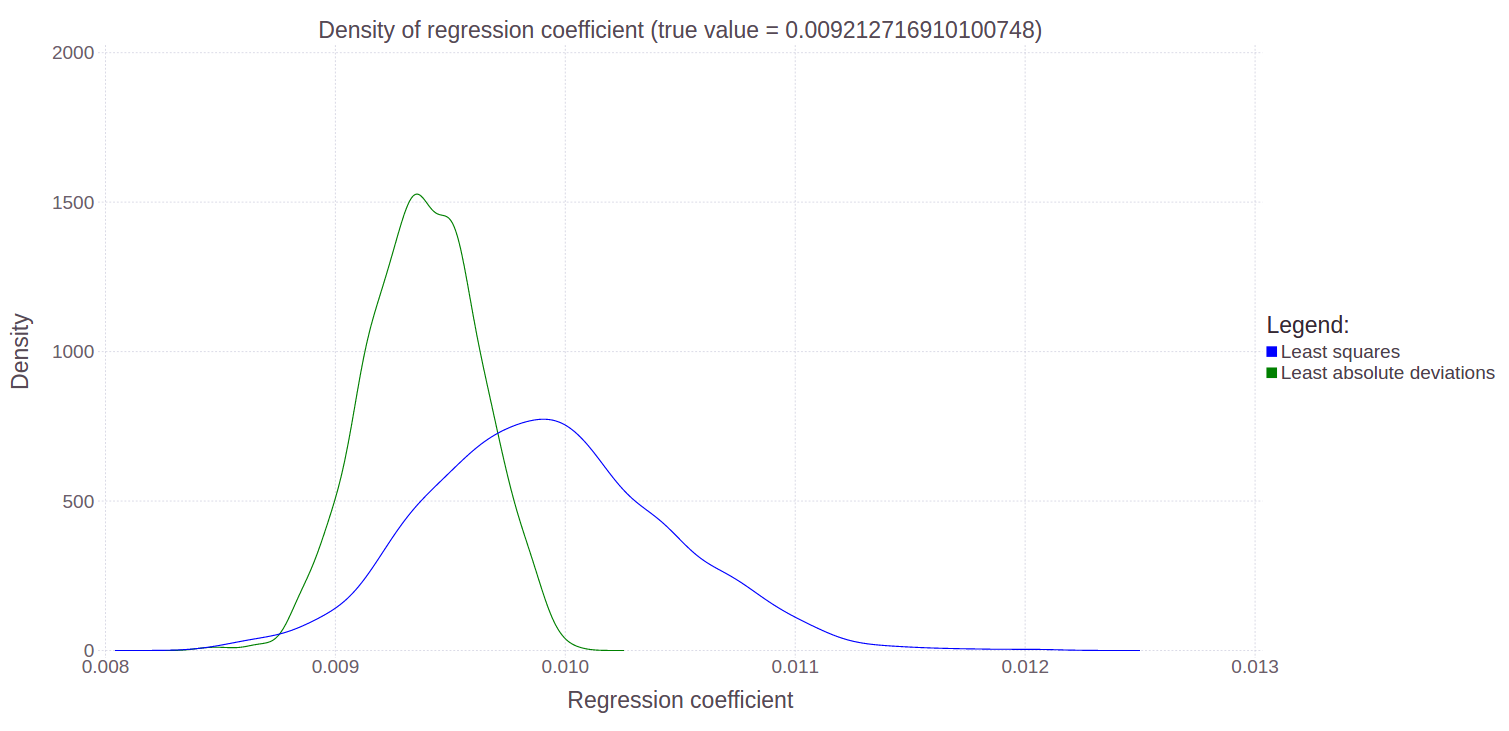
\includegraphics[height=5.35cm]{CoefDensity.png}
\caption{\footnotesize{Regression coefficient sampling distribution.}}
\label{figCoefDensity}
\end{figure}



An interesting question for active portfolio managers is whether this increased estimation accuracy translates into better returns in an active management framework. To answer this question, I conduct a very simple trading simulation. Specifically, I assume an economy with 20 assets, plus a cash asset that earns no interest. The returns for all 20 assets are simulated using the process described earlier in this section,\footnote{Although I significantly reduce the $R^2$ to keep the terminal wealth numbers realistic.} and the returns on the assets are uncorrelated. The portfolio manager is assumed to have access to the signal $s_t$ for all 20 assets, and to know the true functional form of \eqref{retModel}, but not the true values for $\a$ and $\b$. The portfolio manager estimates $\a$ and $\b$ using either OLS or LAD on data from the first half of the sample. Then, for the second half of the sample, in every period $t$, the portfolio manager will go long any asset (with equal weighting) where the forecast return $\hat{r}_t = \hat{\a} + \hat{\b} s_t$ is greater than zero. There are no transaction costs or volume constraints, and starting wealth is 1 million dollars.

The above simulation is repeated $M$ times, and the kernel density estimate of the distribution of terminal wealth given OLS versus LAD are provided in Figure~\ref{figTradingSimTerminalVal}. As can be seen, significant material gains are realised by the portfolio manager who uses LAD instead of OLS.

\begin{figure}[htbp]
\centering
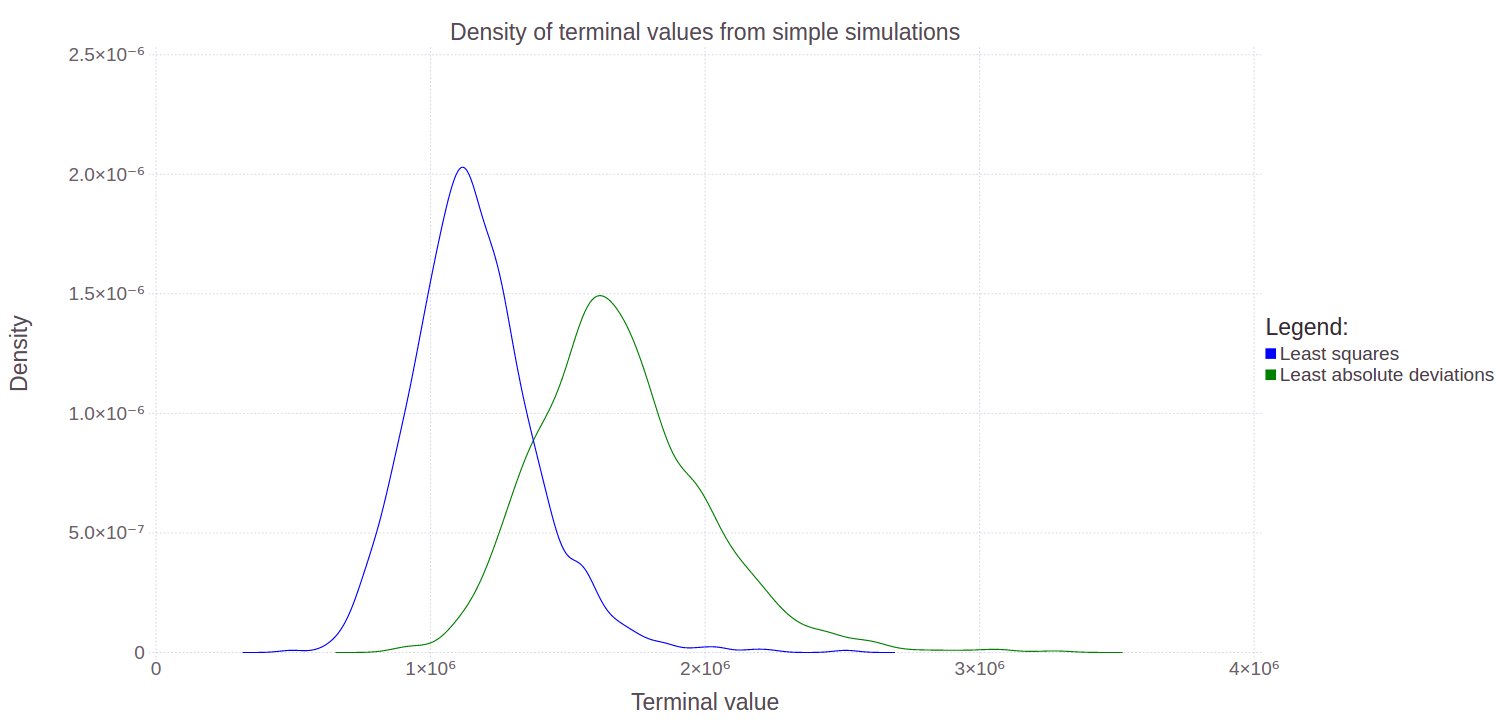
\includegraphics[height=5.35cm]{TradingSimTerminalVal.png}
\caption{\footnotesize{Portfolio terminal value.}}
\label{figTradingSimTerminalVal}
\end{figure}






\section{Conclusion}

In this paper I have introduced the topic of robust statistics, discussed ways of measuring tail fatness, and then investigated the efficacy of several popular robust estimators when used with financial data. The general conclusion suggested in this paper is that the heteroskedasticity present in financial returns is sufficient to justify, at the very least, the consideration of robust methodologies when working with financial data.




%------------------------- BIBLIOGRAPHY -----------------------------------------
\clearpage
%\bibliographystyle{harvard}
%\bibliographystyle{myagsm}
\bibliography{/home/colin/Dropbox/Articles_Academic/BiBTeX/BiBTeX_Article_List}
%

\end{document}
